\documentclass[11pt,a4paper]{article}
\usepackage[margin=2.2cm]{geometry}
\usepackage{amsmath,amssymb}
\usepackage{tikz}
\usepackage{enumitem}
\usepackage{graphicx}
\usepackage[hidelinks]{hyperref}
\setlength{\parindent}{0pt}
\setlength{\parskip}{4pt}
\pagestyle{empty}

\newcounter{ex}
\newenvironment{exercise}[1]{\refstepcounter{ex}\par\medskip
  {\large\bfseries Exercise \theex\ --- #1}\par\smallskip}{\par\medskip}

\begin{document}

\begin{minipage}{0.7\textwidth}
  {\LARGE\bfseries Calculus --- Exercise sheet}\par\smallskip
  Optimization and study of functions
\end{minipage}\hfill
\begin{minipage}{0.25\textwidth}\raggedleft
  
\includegraphics[width=1.6cm]{../../branding/logo-512.png}
\end{minipage}
\par\medskip\hrule\medskip

Solve each exercise on the worksheet, showing every step. Justify your answers.

\begin{exercise}{The best rectangle in a semicircle}
Among all rectangles inscribed in a semicircle of radius $1$, with the base on the
diameter, which one has the largest area? How much is that area?

\begin{center}
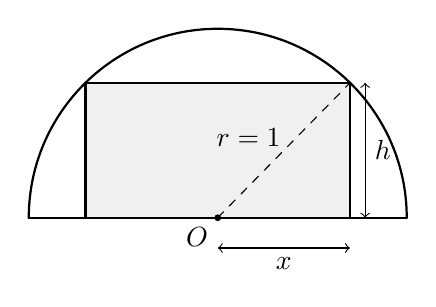
\begin{tikzpicture}[scale=2.4, line cap=round]
  \def\a{0.7}
  \pgfmathsetmacro{\h}{sqrt(1-\a*\a)}
  \fill[gray!12] (-\a,0) rectangle (\a,\h);
  \draw[thick] (-1,0) -- (1,0);
  \draw[thick] (1,0) arc[start angle=0, end angle=180, radius=1];
  \draw[thick] (-\a,0) rectangle (\a,\h);
  \draw[dashed] (0,0) -- (\a,\h);
  \fill (0,0) circle[radius=0.018] node[below left] {$O$};
  \draw[<->] (0,-0.16) -- node[below] {$x$} (\a,-0.16);
  \draw[<->] (\a+0.08,0) -- node[right] {$h$} (\a+0.08,\h);
  \node[above left, inner sep=1pt] at (0.5*\a,0.5*\h) {$r=1$};
\end{tikzpicture}
\end{center}
\end{exercise}

\begin{exercise}{Study of a function}
Consider the function $f(x) = x^3 - 3x$.
\begin{enumerate}[label=\alph*)]
  \item Find the domain of $f$ and check whether $f$ is even or odd.
  \item Find the zeros of $f$.
  \item Compute $f'(x)$ and find the critical points of $f$.
  \item Determine the intervals where $f$ is increasing or decreasing, and its local
        maxima and minima.
  \item Sketch the graph of $f$.
\end{enumerate}
\end{exercise}

\begin{exercise}{Critical points in two variables}
Consider the function $g(x,y) = x^2 - y^2$.
\begin{enumerate}[label=\alph*)]
  \item Compute the partial derivatives $\dfrac{\partial g}{\partial x}$ and
        $\dfrac{\partial g}{\partial y}$.
  \item Find the critical points of $g$.
  \item Is each critical point a local maximum, a local minimum or a saddle point?
\end{enumerate}
\end{exercise}

\end{document}
